\documentclass[fleqn]{article}
\author{MODFLOW Development Team}

\usepackage{natbib}
\usepackage{amsmath}
\usepackage{bm}
\usepackage{xcolor}
\usepackage{graphicx}

\graphicspath{{./figures/}}
\newcommand{\matr}[1]{\mathbf{#1}}
\DeclareMathOperator{\sign}{sign}

\begin{document}

\title{Surface Water Flow in MODFLOW 6}
\maketitle

\tableofcontents

\section{Introduction}
The Surface Water Flow (SWF) Model simulates one-dimensional channel flow and two-dimensional overland flow using the diffusive-wave approximation to the Saint-Venant equations.  The SWF Model is integrated into the MODFLOW 6 framework as a new type of supported model.  An SWF Model can be run by itself in a MODFLOW 6 simulation or it can be coupled with a Groundwater Flow (GWF) Model using an SWF-GWF Exchange.

There are three different types of discretization packages that can be used with the SWF Model.  These include 

\begin{itemize}
  \item Discretization by Vertices in One Dimension (DISV1D), 
  \item Discretization by Vertices in Two Dimensions (DISV2D), and
  \item Structured Discretization in Two Dimensions (DIS2D).
\end{itemize}

\noindent For SWF Models that simulate one-dimensional channel flow, the DISV1D Package must be used.  For SWF models that simulate two-dimensional channel flow, either the DIV2D or DIS2D Packages must be used.  Because an SFW Model can use only one discretization package, an SWF Model must be either a channel model or an overland flow model.  More than one SWF Model can be used in a simulation.

In addition to the discretization package, the SWF Model supports other required and optional packages as shown in table \ref{table:ftype-swf}.

\begin{table}[ht]
   \caption{Packages that can be activated and used with the Surface Water Flow (SWF) Model.}
   \begin{tabular*}{\columnwidth}{l l l}
   \hline
   \hline
   File Type & Input File Description & Multi-Package \\
   \hline
   DISV1D6 & Discretization by Vertices in One Dimension \\
   DISV2D6 & Discretization by Vertices in Two Dimensions \\
   DIS2D6 & Structured Discretization in Two Dimensions \\
   IC6 & Initial Conditions \\
   OC6 & Output Control \\
   DFW6 & Diffusive Wave \\ 
   STO6 & Storage \\
   CHD6 & Time-Variant Specified Head & * \\
   FLW6 & Specified Flow & * \\
   ZDG6 & Zero-Depth Gradient Outflow &   \\
   CDB6 & Critical-Depth-Boundary Outflow &   \\
   OBS6 & Observations \\
   \hline 
   \end{tabular*}
   \label{table:ftype-swf}
%   \end{center}
%   \normalsize
  \end{table}


\section{Mathematical Model}
Following~\cite{panday2004} and~\cite{hughes2012documentation} the partial differential equation for the the diffusive wave approximation to the full St. Venant equations can be written for both one-dimensional channel flow and two-dimensional overland flow.  In both cases, flow is based on Manning's equation, which can be expressed as

\begin{equation}
  Q = \frac{1}{n} A R^{\frac{2}{3}} \sqrt{S_f},
  \label{eqn:manning}
\end{equation}

\noindent where Q is the volumetric flow rate in $L^3/T$, $n$ is the Manning's roughness coefficient in $T/L^{1/3}$, $A$ is the area perpendicular to flow ($L^2$), $R$ is the hydraulic radius ($L$) defined as the area divided by the wetted perimeter, and $S_f$ is the friction slope (dimensionless).

The following equation is for one-dimensional channel flow,

\begin{equation}
  \frac{\partial}{\partial \ell}
  \left (
  \frac{A R^{\frac{2}{3}}}{n \left | \frac{\partial h}{\partial \ell} \right |^{\frac{1}{2}} } \frac{\partial h}{\partial \ell}
  \right )
  + Q_s'
  =   
  \frac{\partial A}{\partial t},
\label{eqn:onedpd}
\end{equation}

\noindent where $\ell$ is the length ($L$) along the channel, $A$ is the cross-sectional area  ($L^2$) for flow, $R$ is the hydraulic radius ($L$) defined as the flow area divided by the wetted perimeter, $n$ is the Manning's roughness coefficient ($T/L^{\frac{1}{3}}$), $h$ is the water surface elevation ($L$), $Q_s'$ is a source term representing the volumetric flow rate of a source per length of channel ($L^2/T$), and $t$ is time ($T$). 

For two-dimensional overland flow, the partial differential equation can be written as

\begin{equation}
  \frac{\partial}{\partial x}
  \left (
  \frac{d^{\frac{5}{3}}}{n \left | \frac{\partial h}{\partial s} \right |^{\frac{1}{2}} } \frac{\partial h}{\partial x}
  \right )
  + \frac{\partial}{\partial y}
  \left (
  \frac{d^{\frac{5}{3}}}{n \left | \frac{\partial h}{\partial s} \right |^{\frac{1}{2}} } \frac{\partial h}{\partial y}
  \right )
  + q_s
  = \frac{\partial h}{\partial t},
  \label{eqn:twodpd}
\end{equation}

\noindent where $x$ and $y$ are the two-dimensional coordinate directions, $d$ is the water depth ($L$), $s$ is the coordinate direction corresponding to the maximum water surface slope ($L$), and $q_s$ is a source term, in dimensions of $L/T$, representing the volumetric rate of source water per unit area.

Due to the dimensionality difference between one-dimensional channel flow and two-dimensional overland flow, the dimensions of the terms in equations~\ref{eqn:onedpd} and~\ref{eqn:twodpd} are different.  Equation~\ref{eqn:onedpd} has dimensions of $L^2/T$ whereas equation~\ref{eqn:twodpd} has dimensions of $L/T$.

\section{Numerical Model}
The surface water flow equation in MODFLOW 6 is discretized using a control-volume finite-difference (CVFD) method. This section describes the equations formulated by the SWF model, discretization options, and the general forms of the finite-difference equations used to simulate channel and overland surface water flow.

\subsection{Control-Volume Finite-Difference Equation}
Equations~\ref{eqn:onedpd} and~\ref{eqn:twodpd}, together with initial conditions and any relevant boundary conditions, represents mathematically the surface water flow balance at any point in the model domain. In certain simple cases, equations~\ref{eqn:onedpd} and~\ref{eqn:twodpd} can be solved analytically to obtain a mathematical expression for water surface elevation and flow throughout a model domain. The balance of surface water flow is formulated for each model cell, taking into account the flows of water to and from neighboring cells, the flow of water to and from cells in a connected surface water model, the flow of water to and from cells in a connected groundwater model, boundary outflows, as well as flows to or from external sources and sinks, and changes in storage.  The general control-volume finite-difference (CVFD) equation for both channel and overland flow is expressed as

\begin{equation}
  \label{eqn:cvfd}
  \begin{split}
  \sum \limits_{m \in \eta_{n}} Q_{n,m}^{SWF}
  + \sum \limits_{iss=1}^{NSS_n} Q_{n,iss}^{SS}
  + Q_n^{ZDG}
  + Q_n^{CDB}
  - Q_{STO} \\
  + \sum \limits_{m \in S_{n}} Q_{n,m}^{SWF-SWF}
  + \sum \limits_{m \in G_{n}} Q_{n,m}^{SWF-GWF}
  = 
  0,
  \end{split}
\end{equation}

\noindent where 
$\eta_{n}$ is a list of the surface water cells in the model that are connected to cell $n$, 
$Q_{n,m}^{SWF}$ is the flow into cell $n$ from cell $m$ ($Q_{n,m}^{SWF}$ is negative if flow is from cell $n$ to cell $m$) with dimensions of L$^{3}$T$^{-1}$, 
$NSS_n$ is the number of sources or sinks in cell $n$, $Q_{n,iss}^{SS}$ is the flow rate for source or sink $iss$, 
$Q_n^{ZDG}$ is the outflow from cell $n$ for a zero-depth-gradient condition, 
$Q_n^{CDB}$ is the outflow from cell $n$ for a critical-depth-boundary condition,
$Q_{STO}$ is the change in the volume of water stored in cell $n$,
$S_{n}$ is a list of the cells in another surface water model that are connected to cell $n$,
$Q_{n,m}^{SWF-SWF}$ is the flow into cell $n$ from cell $m$, 
$G_{n}$ is a list of the cells in an underlying groundwater model that are connected to cell $n$,
and $Q_{n,m}^{SWF-GWF}$ is the flow into cell $n$ from cell $m$.  
All of the flow terms in equation \ref{eqn:cvfd} have dimensions of L$^{3}$T$^{-1}$.

Taken together, the surface water flow balance equations for all the cells form a system of linear equations that is solved iteratively using a linear matrix solver. Details of the individual terms and the CVFD implementation in the SWF Model are described below.

\subsection{Characteristics of a Model Cell}
The characterics of a model cell are different depending on whether the model represents channel flow or overland flow.  For one-dimensional channels, surface water flows through a network of connected model cells.  Model cells are one dimensional in plan view but can have different cross-sectional geometries.  The default cross-sectional geometry corresponds to a hydraulically wide rectangular channel in which there is no resistance to flow along the vertical sides.  If the default channel configuration does not represent field conditions, then the Cross Section (CXS) Package can be activated and used to provide more detailed cross-section information.

Two-dimensional overland flow is modeled on a structured or unstructured grid.  For each cell, the SWF Model calculates the water surface elevation for the cell and for flow between each model cell and its neighbors.  Resistance to flow occurs through a Manning's roughness coefficient.

\subsection{Connections Between Cells}
A connection between two cells indicates that the cells are in hydraulic communication and that surface water can flow between the cells under the influence of a hydraulic gradient.  Cell connections are calculated by the SWF Model using information about the channel network or the overland flow grid.  For channel (DISV1D) and two dimensional vertex (DISV2D) grids, cell connectivity is determined by the presence of shared vertices.  For a structured two-dimensional grid (DIS2D), each cell is hydraulically connected to the four surrounding cells.  

For accurate solutions with the CVFD method, there are geometric requirements regarding cell connections.  First, a line drawn between the centers of any two connected cells should intersect the shared face at a right angle. Second, the intersection point should coincide with an appropriate mean position on the shared face \cite{narasimhan1976integrated}.  The smaller the deviation from these CVFD connection requirements, the smaller the loss in accuracy in the surface water flow solution. 

\subsection{Model Grids}
The SWF Model supports two different types of discretization approaches: a one-dimensional channel network and a two-dimensional overland flow grid.  The two-dimensional overland flow grid may use either a structured grid consisting of rows and columns or an unstructured grid specified using vertices and cells that are defined using those vertices.  A SWF Model must use either the one-dimensional channel network or the the two-dimensional overland flow discretization approaches.  

\subsubsection{One-Dimensional Channel Flow}
A one-dimensional channel network is represented using the Discretization by Vertices in One Dimension (DISV1D) Package.  An example of a channel network is shown in figure~\ref{fig:channel_network}.  The channel network is discretized into reaches.  The SWF Model solves for the water level in reach by balancing the flows between reaches with storage changes and sources.  Stage calculation points within a reach are typically located halfway between the reach starting and ending vertices; however, the user may adjust the stage calculation point in either direction (toward or away from the first reach vertex), which can be advantageous in some situations.  A reach is connected to another reach when they share a vertex.  Reaches do not need to be defined in any particular order.  If a reach terminates at a vertex and that vertex is not shared by another reach, then by default, there is no outflow from the ending vertex location.  If the user intends for outflow to occur, then a stress package must be activated and assigned to that reach.

\begin{figure}
  \centering
  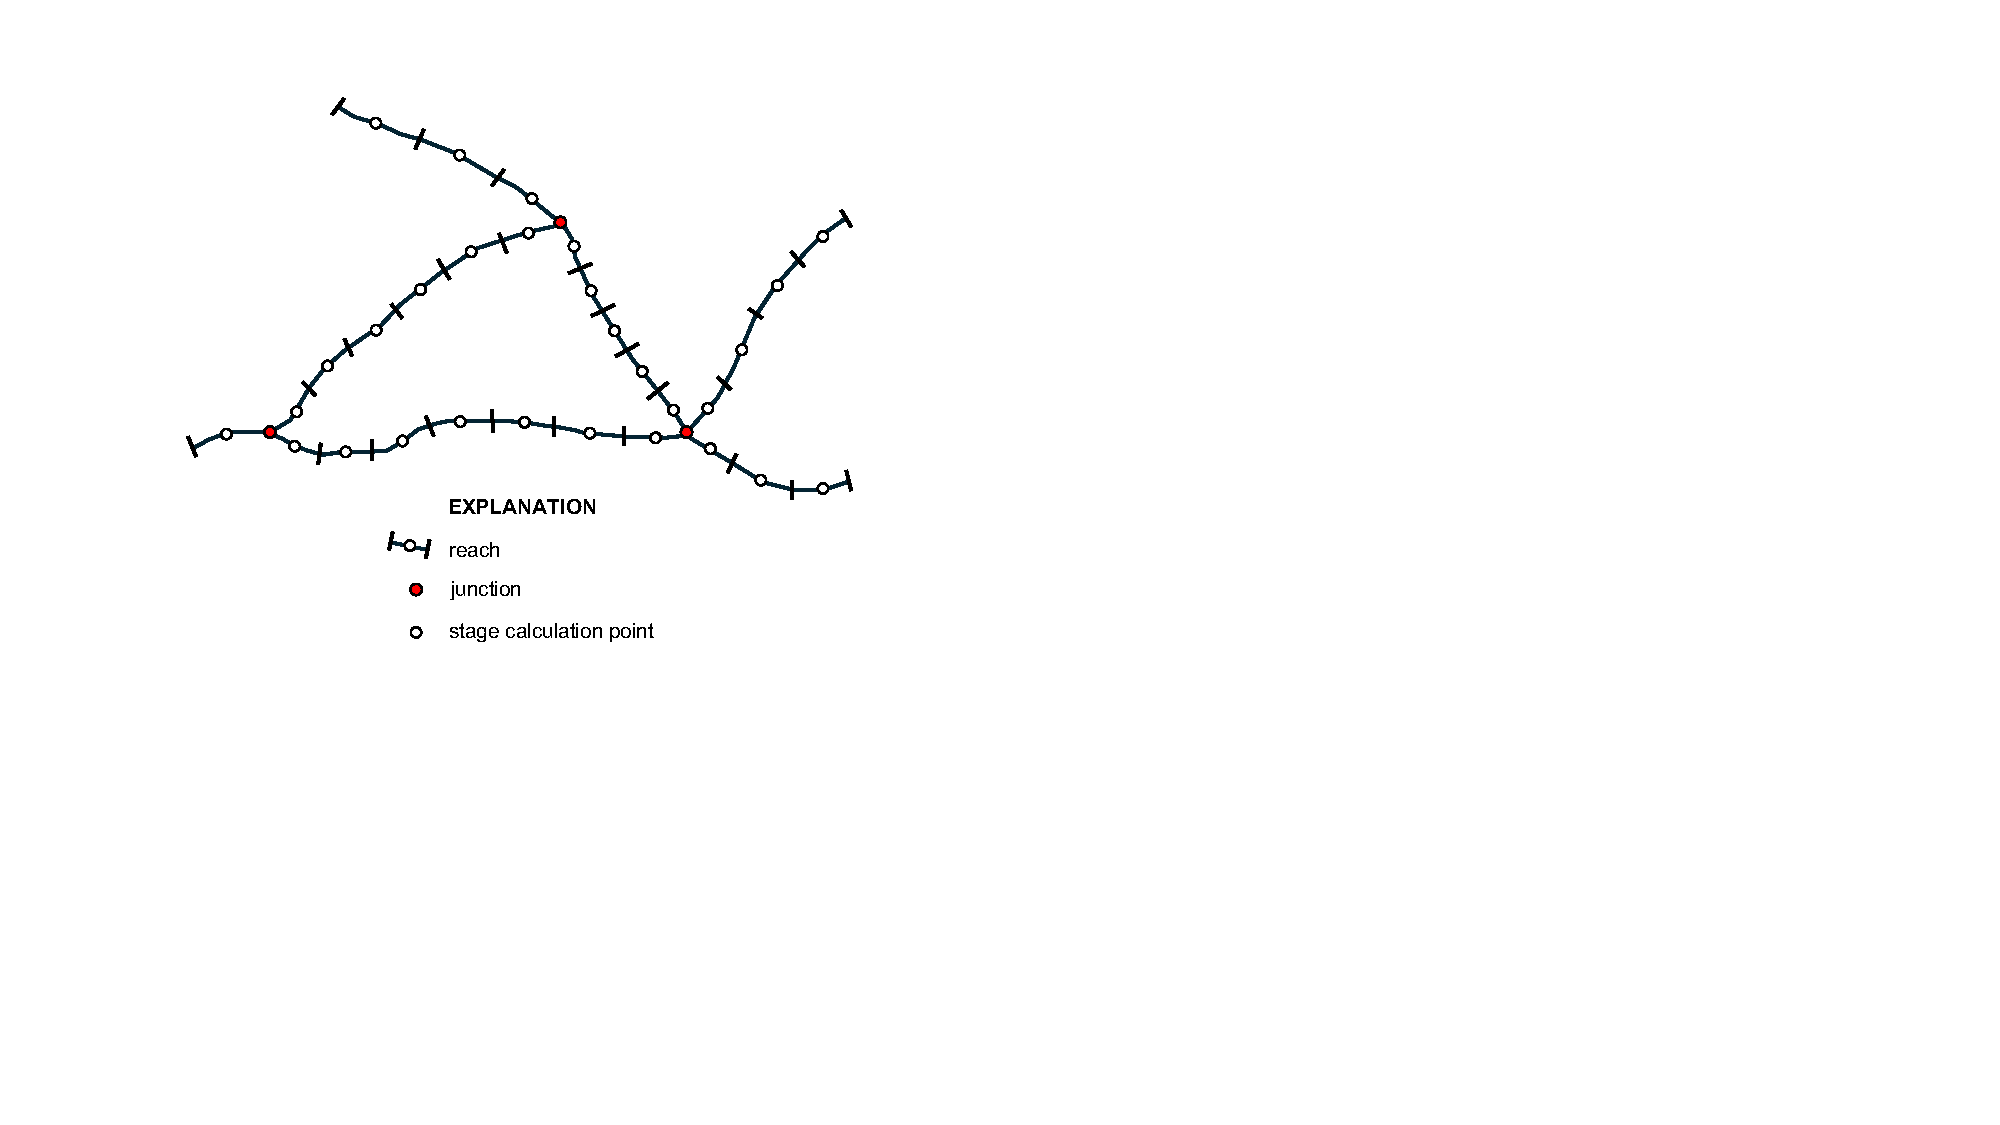
\includegraphics[scale=0.9]{figures/channel_network.pdf}
  \caption[Schematic showing a channel network.]{Schematic showing a channel network.  The channel network is discretized by the user into reaches.  Stage is calculated within the reach at stage calculation points.  Stage calculations are typically located halfway between the reach start and reach end vertices, however, the user can adjust the fractional position of the stage calculation point along the reach.}
  \label{fig:channel_network}
\end{figure}
  
\subsubsection{Two-Dimensional Overland Flow}
Two-dimensional overland flow can be represented using either the regular structured grid discretization (DIS2D) Package or the unstructured discretization by vertices (DISV2D) Package.  These two discretization types are patterned after their Groundwater Flow (GWF) Model counterparts, DIS and DISV, respectively.  The difference between the SWF overland flow discretization types and the GWF Model discretization types is that the SWF versions are two dimensional and do not have a top defined or multiple layers.

For DIS2D grids, stage calculation points are located in the center of the model cell.  For DISV2D grids, stage calculation points are assigned by the user; they should generally be located in the center of the cell, but there is flexibility to adjust them spatially to better represent precise boundary locations.  By default, the model domain boundary represents no-flow conditions.  Outflow conditions must be activated by assigning a stress package to the desired locations.

\subsubsection{Channel Cross Sections}

For SWF Models defined to represent channel flow (those models that use the DISV1D discretization package), each cell is characterized by a cross-section geometry.  By default, a channel is assigned a rectangular cross-section with a width provided by the user.  With the default cross-section geometry, the channel is treated as hydraulically wide with the wetted perimeter set equal to the channel width (Figure \ref{fig:cxs}a).

Users may also define more detailed cross-section geometries using the Cross Section (CXS) Package.  Examples of cross-section geometries are shown in Figure \ref{fig:cxs}b--d.

Users may also define different Manning's roughness coefficients for each segment within a cross section, as shown in Figure \ref{fig:cxs_rough}.

% This figure below is for the case where roughness is the same for every line segment in the cross section 
\begin{figure}[h!tbp]
	\centering
	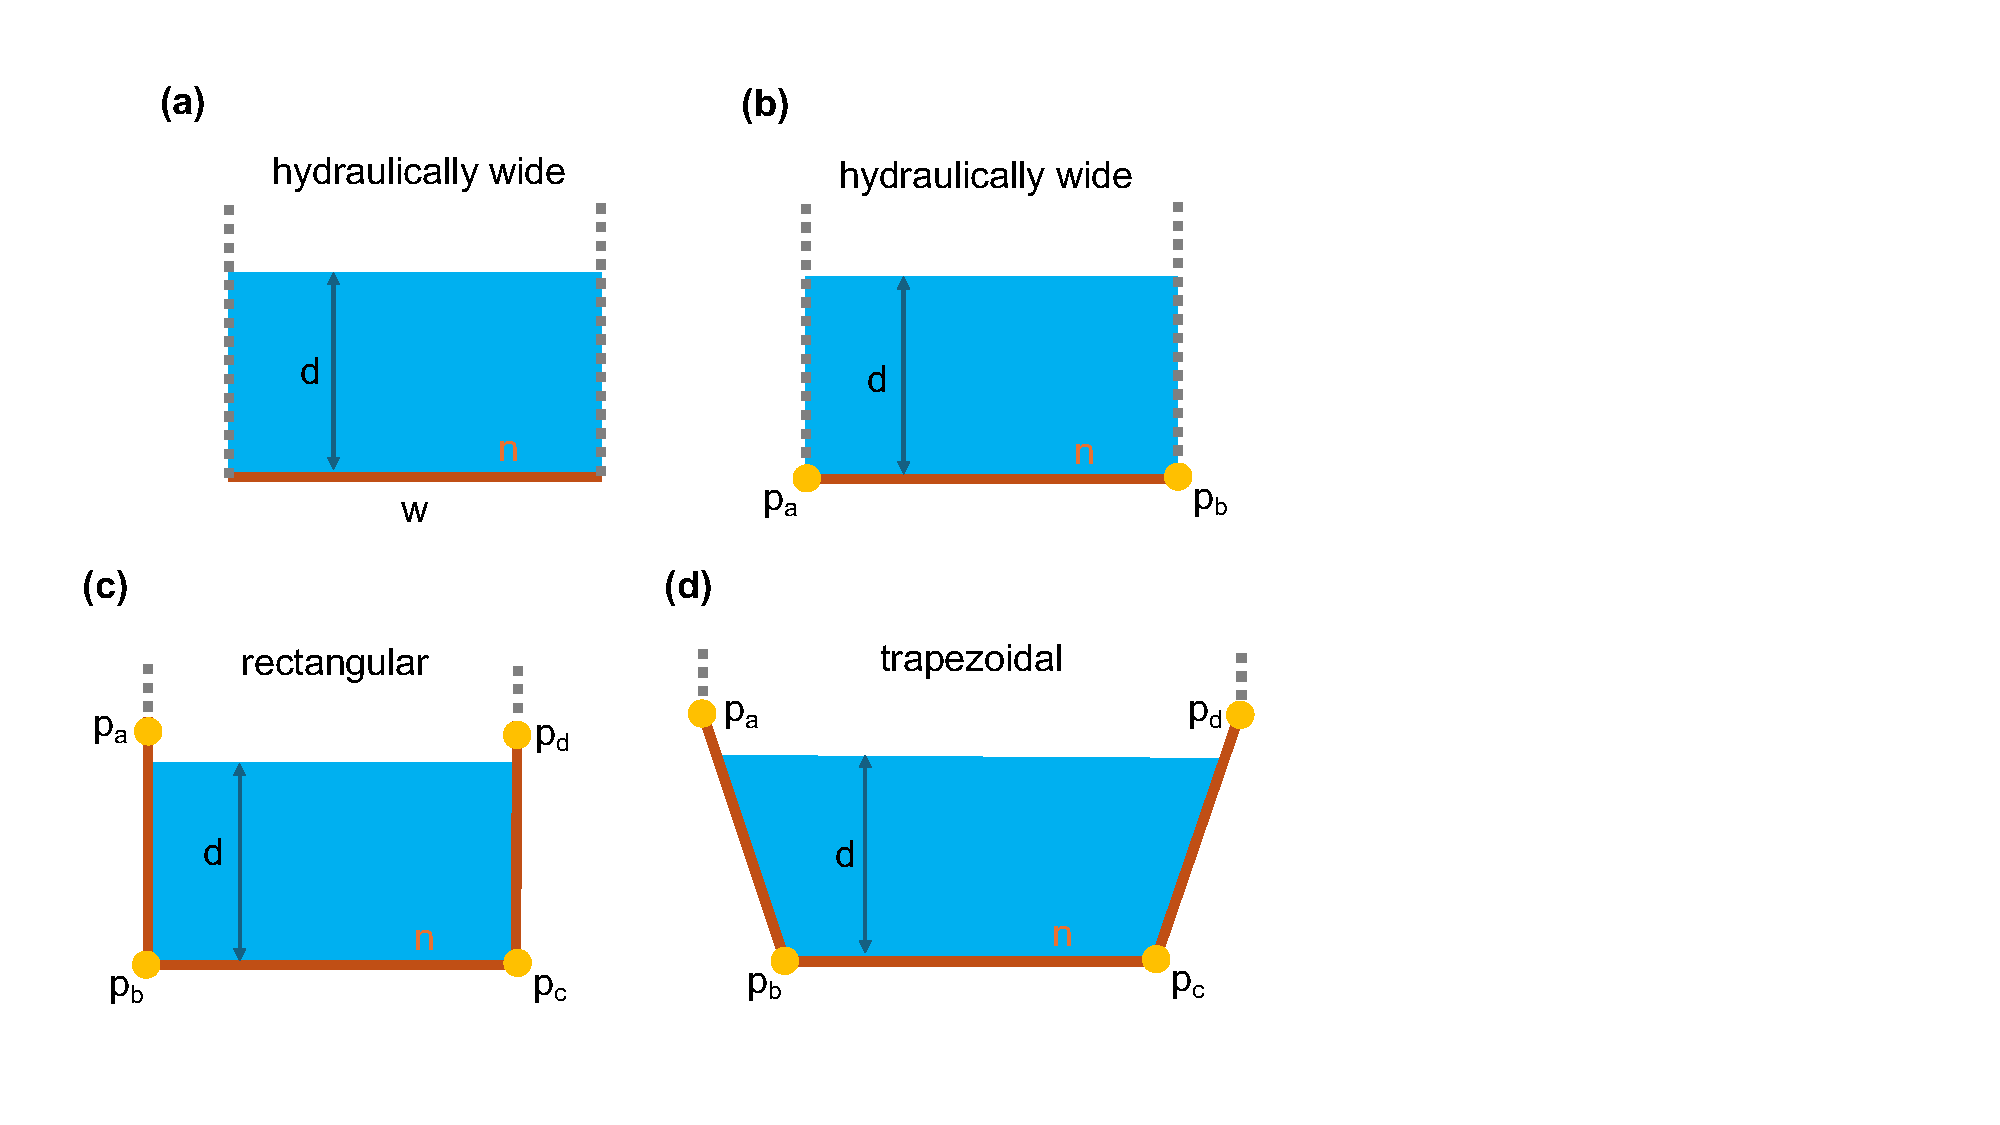
\includegraphics[scale=0.5]{figures/cxs.pdf}
	\caption[Schematic showing different types of channel cross sections with constant roughness.]{Schematic showing different types of cross sections with a single Manning's roughness coefficient $n$: (a) hydraulically wide cross section defined using the width input parameter; (b) hydraulically wide cross section defined using two points; (c) a rectangular cross section defined using four points, and (d) a trapezoidal cross section defined using four points.  For the hydraulically wide rectangular cross sections in (a) and (b) the model does not include any channel resistance for the vertical wetted sections corresponding to the dashed lines.  For cross sections shown in (c) and (d), if the water surface rises above the channel points, no channel resistance is included for sections above the uppermost points}
	\label{fig:cxs}
\end{figure}

% This figure below is for the case where roughness varies for each line segment in the cross section 
\begin{figure}[h!tbp]
	\centering
	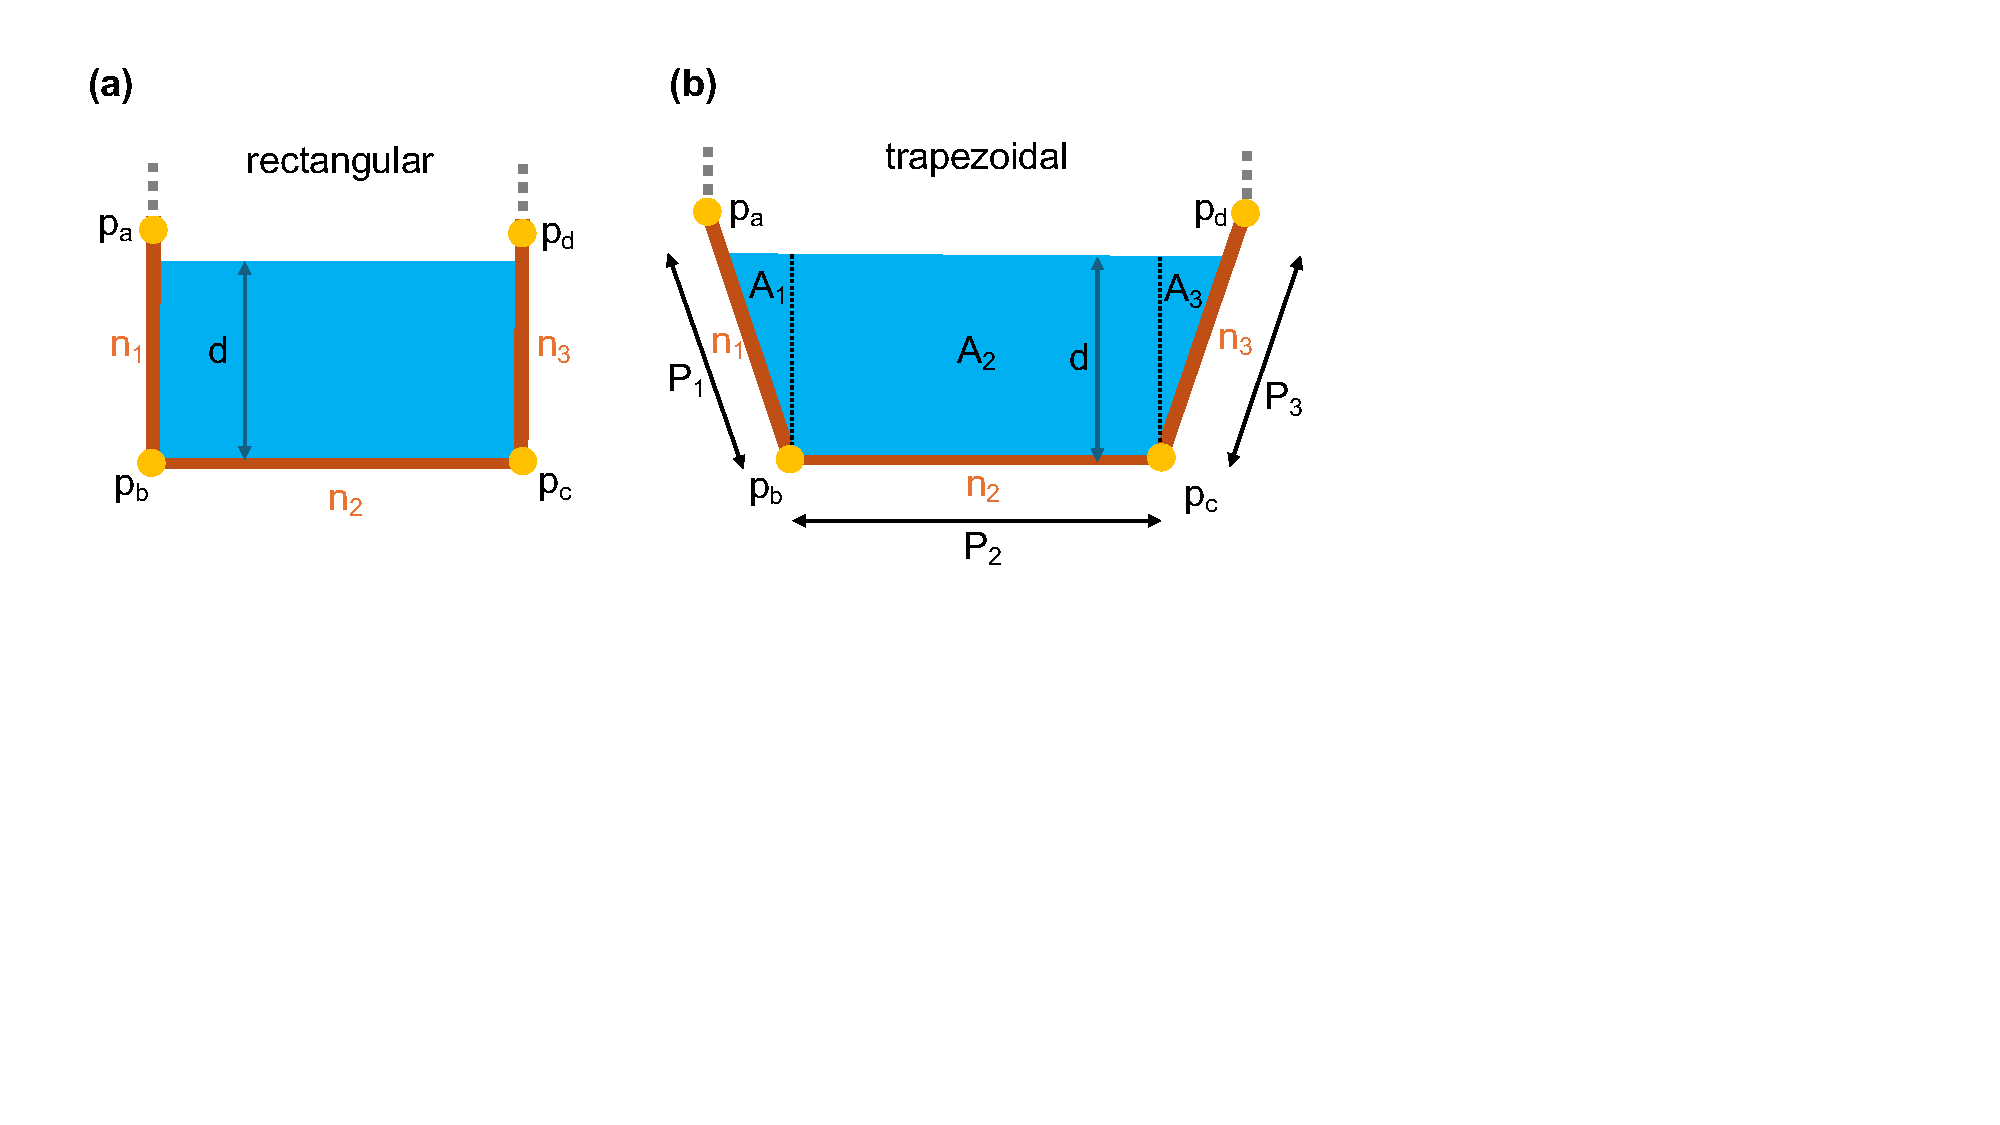
\includegraphics[scale=0.5]{figures/cxs_rough.pdf}
	\caption[Schematic showing different types of channel cross sections with variable roughness.]{Schematic showing different types of cross sections with variable Manning's roughness coefficient: (a) a rectangular cross section defined using four points, and (b) a trapezoidal cross section defined using four points.  The Manning's roughness coefficient varies by line segment.  If the water surface rises above the channel points, no channel resistance is included for sections above the uppermost points}
	\label{fig:cxs_rough}
\end{figure}

\subsection{Internal Flows}
Flows between cells, whether they are channel cells or overland flow cells, are called ``internal flows.'' An internal flow between two cells $n$ and $m$ is denoted by $Q_{n,m}^{SWF}$.  The sum of internal flows is shown as the first term in the CVFD equation (equation \ref{eqn:cvfd}).  Internal flows between cells are calculated using a form of Manning's equation in which flow area and hydraulic radius are calculated from the simulated depth in the cells, and the friction slope is calculated based on the head difference between cells.  

% The following is a general expression for Manning's equation:

% \begin{equation}
%   Q = \frac{1}{n} A R^{\frac{2}{3}} \sqrt{S_f},
% \end{equation}

% \noindent where $R$ is the hydraulic radius ($L$) equal to the flow area divided by the wetted perimeter, and $S_f$ is the water surface slope (dimensionless). 

For the numerical implementation in the SWF Model, Manning's equation is expressed as a product of a conductance term and the head difference between cells $n$ and $m$:

\begin{equation}
  Q_{nm}^{SWF} = \overline{C}_{nm} \left ( h_m - h_n \right ).
\end{equation}

\noindent The conductance-based flow expression allows individual cell conductances to be calculated for each of the two connected reaches and then averaged together to give a representative conductance for the connection.  The representative conductance between reach $n$ and reach $m$ ($\overline{C}_{nm}$) is calculated by averaging a conductance for reach $n$ with a conductance for reach $m$.  The conductance for reach $n$, denoted by $C_{nm}$ ($L^2/T$), is calculated over the distance from the stage calculation point of $n$ to its shared face with cell $m$.  Likewise, the conductance for reach $m$, over the distance between the stage calculation point for $m$ and its shared face with cell $n$ is denoted by $C_{mn}$ and also has dimensions of $L^2/T$.

The average conductance between reach $n$ and reach $m$ is calculated using the harmonic mean of $C_{nm}$ and $C_{mn}$ to give

\begin{equation}
  \overline{C}_{nm} = \frac{C_{nm}  C_{mn}}{C_{nm} + C_{mn}}.
\end{equation}

\noindent The harmonic mean preferentially weights the average toward the lower of the two values and is based on piecewise constant reach properties that may change abruptly at the face between different reaches.

The conductance for reach $n$ in the $m$ direction ($C_{nm}$) can be expressed as

\begin{equation}
  C_{nm} = 
  \frac{
  A_n 
  R_{n}^{\frac{2}{3}}
  }
  {n_n
  L_{nm}
  \sqrt{| \gamma_n |}
  },
\label{eqn:cn}
\end{equation}

\noindent where $A_n$ is the cross-sectional flow area ($L^2$) for reach $n$ calculated as a function of the water depth, $R_n$ is the hydraulic radius ($L$) for reach $n$, which is the cross-sectional flow area divided by the wetted perimeter, calculated as a function of the water depth, $n_n$ is the Manning's roughness coefficient ($T/L^{\frac{1}{3}}$) for reach $n$, $L_{nm}$ is the distance ($L$) from the stage calculation point in cell $n$ to the shared edge with reach $m$, and $\gamma_n$ is the hydraulic gradient ($L^0$) for reach $n$.

Several of the terms in equation \ref{eqn:cn} are combined into a single term for reach $n$ called channel conveyance ($\kappa_n$), which is defined as

\begin{equation}
  \kappa_n = \frac{A_n R_n^{\frac{2}{3}}}{n_n}.
\label{eqn:conveyance}
\end{equation}

\noindent Channel conveyance for reach $n$ is calculated as a function of an upstream-weighted water depth.  Thus, channel conveyance for reach $n$ can be written as

\begin{equation}
  \kappa_n = \frac{A_n (d_u) R_n (d_u) ^{\frac{2}{3}}}{n_n},
\label{eqn:conveyancedu}
\end{equation}

\noindent where the $A_n$ and $R_n$ terms include $(d_u)$ to indicate that they are calculated as a function of $d_u$.  $d_u$ is assigned to the depth of the reach (either from cell $n$ or cell $m$) with the higher stage:

\[
d_u = 
\begin{cases}
  d_n & \text{if $h_n>h_m$} \\
  d_m & \text{otherwise}
\end{cases}.
\]

With this definition for channel conveyance, equation \ref{eqn:cn} can be simplified as

\begin{equation}
  C_{nm} = 
  \frac{
  \kappa_n 
  }
  {
  L_{nm}
  \sqrt{| \gamma_n |}
  },
\label{eqn:cn2}
\end{equation}

Channel conveyance is calculated in several different ways depending on how a cross section is defined for a reach.  For the cross sections shown in figure \ref{fig:cxs} a single Manning's roughness coefficient is assigned for the entire section.  If a single Manning's roughness coefficient is used to define the entire section for reach $n$, then the channel conveyance is calculated according to equation \ref{eqn:conveyance}.  If a cross section does not have a constant Manning's roughness coefficient for all line segments that define the channel, as shown for example in Figure \ref{fig:cxs_rough}, then a composite conveyance is calculated by summing the individual conveyance parts for the channel as

\begin{equation}
  \kappa_n = \sum_{i=1}^{NLS} \frac{A_{n,i} \left ( \frac {A_{n,i}}{P_{n,i}}\right )^{\frac{2}{3}}}{n_{n,i}},
\end{equation}

\noindent where $NLS$ is the number of line segments used to define the channel cross section.


\subsection{Sources and Sinks}

The SWF Model supports the addition or removal of water to or from an individual reach using the specified flow (FLW) Package.  


\subsection{Boundaries}
The SWF Model supports two types of outflow boundaries.  These include the Zero-Depth Gradient (ZDG) Package and the Critical-Depth Boundary (CDB) Package.  The SWF Model also supports a Constant-Head Boundary (CHD) Package.


\subsubsection{Zero-Depth Gradient Package}

The zero-depth-gradient outflow condition uses Manning's equation and the calculated stage in the cell to determine the volumetric outflow rate, $Q_{n}^{ZDG}$, in dimensions of $L^3/T$ as

\begin{equation}
  Q_{n}^{ZDG} = 
  \kappa_{n,izdg} \left ( d_n \right ) \sqrt{S_0},
\label{eqn:qzdg}
\end{equation}

\noindent where $\kappa_{n,izdg}$ is conveyance ($L^3/T$) calculated for cell $n$ using the properties specified by the user for the zero-depth-gradient condition $izdg$.  The conveyance $\kappa_{n,izdg}$ is calculated as

\begin{equation}
  \kappa_{n,izdg} = \frac{A_{izdg} (d_n) R_{izdg} (d_n)^{\frac{2}{3}}}{n_{izdg}},
\label{eqn:conveyancezdg}
\end{equation}

\noindent where $A_{izdg} (d_n)$ is the flow area ($L^2$) calculated for the channel or overland flow cell using the smoothed cell depth $(d_n)$, $R_{izdg} (d_n)$ is the hydraulic radius ($L$) calculated for the channel or overland flow cell using the smoothed cell depth $(d_n)$, and $n_{izdg}$ is the Manning's roughness coefficient ($T/L^{1/3}$) specified by the user for the $izdg$ condition.  

For channels, the flow area and hydraulic radius are calculated using the cross-section geometry specified for cell $n$.  If a cross-section geometry is specified for the channel, then the cross-section geometry is used with the width parameter specified for the zero-depth-gradient condition in the calculation of flow area and hydraulic radius.

\subsubsection{Critical-Depth-Boundary Package}

With the critical-depth condition outflow is calculated such that the simulated depth is equal to the critical depth.  The critical depth is the depth of water that occurs under free-fall conditions, such as at a waterfall or other steep break in bottom surface slope.  The critical-depth-boundary is included by calculating the outflow $Q_{n}^{CDB}$ according to the following equation,

\begin{equation}
  Q_{n}^{CDB} = 
  \left ( g A_{icdb} (d_n)^2 R_{icdb} (d_n) \right )^{1/2},
\label{eqn:qcdb}
\end{equation}

\noindent where $g$ is the constant of acceleration due to gravity ($L^2/T$), $A_{icdb} (d_n)$ is the flow area ($L^2$) calculated for the channel or overland flow cell using the smoothed cell depth $(d_n)$, and $R_{icdb} (d_n)$ is the hydraulic radius ($L$) calculated for the channel or overland flow cell using the smoothed cell depth $(d_n)$.

\subsubsection{Constant Head Package}

The CHD Package can be used to specify the head in a SWF Model cell.  The CHD Package for the SWF Model works the same as the CHD Package for the Groundwater Flow (GWF) Model.  Constant-head cells are those for which the head is specified for each time, and the head value does not change as a result of solving the flow equations. The user may specify a different head value for different time steps, but that head remains fixed for the time step.

\subsection{Storage}

For transient simulations, the storage change within a model cell is calculated as


\subsection{Flow Exchange between Surface Water Models}

Not implemented yet.


\subsection{Flow Exchange between Surface Water and Groundwater Models}

The SWF Model can be connected to an underlying Groundwater Flow (GWF) Model using a SWF-GWF Exchange.  The flow between the SWF and GWF Models is calculated based on the following expression for flow,

\begin{equation}
  Q_{n,m}^{SWF-GWF} = s_{n,m} A_{n,m} \acute{K}_{n,m} (h_m - h_n),
\end{equation}

\noindent where $Q_{n,m}^{SWF-GWF}$ is the volumetric flow rate between a surface water cell $n$ and a groundwater model cell $m$ in $L^{3}$T$^{-1}$, $s_{n,m}$ is a quadratic smoothing factor that ranges from zero when the upstream-weighted water depth is zero to a value of one when the upstream-weighted water depth is greater than or equal to a smoothening depth (presently set as $10^{-6}$), $A_{n,m}$ is the interaction area for flow ($L^2$), $\acute{K}_{n,m}$ is the leakance ($T^{-1}$) of the bed sediments calculated as the hydraulic conductivity of the bed sediments divided the thickness of the bed sediments, and $h_n$ and $h_m$ are the water surface elevation and groundwater head of the surface water cell and groundwater cell, respectively.

The interaction area for flow $A_{n,m}$ is defined differently for channel cells than for overland flow cells.  For channel cells, the interaction area is defined as

\begin{equation}
  A_{n,m} = L_{n,m} P_{up},
\end{equation}

\noindent where $L_{n,m}$ is the length ($L$) of channel $n$ overlying groundwater model cell $m$, and $P_{up}$ is the upstream-weighted wetted perimeter of the channel ($L$) calculated using either $h_n$ or $h_m$, whichever is greater.

For overland flow cells, the interaction area corresponds to the overlapping surface area between the overland flow model cell and the underlying groundwater flow model cell.  This area is provided as input by the user.  If the overland flow model grid in plan view is the same as the groundwater flow model grid, then the interaction area is simply the area of the cell; however, it is possible to use a different grid and so the interaction area must be provided by the user.

\section{Numerical Solution}

The MODFLOW 6 framework is designed to solve one or more numerical models using iterative solution methods \cite{modflow6framework}.  In particular, systems of equations arising from discretized flow equations are often written in matrix form as

\begin{equation}
\label{eqn:axb}
\matr{A h} = \matr{b},
\end{equation}

\noindent where $\matr{A}$ is a matrix of the coefficients of head; $\matr{h}$ is a vector of head values at the end of time step, for all active and constant head cells in the grid; and $\matr{b}$ is a vector of the constant terms for all active and constant head cells in the grid. Assembly of the vector $\matr{b}$ and the terms that comprise $\matr{A}$ occurs through a series of subroutine and method calls by the program. The vector $\matr{b}$ and the terms comprising $\matr{A}$ are then transferred to the solver, which solves the matrix equations for the vector $\matr{h}$. For many flow problems, equation \ref{eqn:axb} is nonlinear in that individual entries in the $\matr{A}$ matrix are a function of head (the dependent variable).  These nonlinearities are resolved through iteration by repeatedly formulating and solving equation \ref{eqn:axb} using $\matr{A}$ matrix entries recalculated using heads from the previous iteration.

The SWF Model was designed to take advantage of the existing linear and nonlinear solution techniques available in the MODFLOW 6 framework.  

\subsection{Overview of the Newton-Raphson Method}

The Newton-Raphson method can be applied to a system of nonlinear equations like those resulting from discretization of the surface water flow equation.  The Newton-Raphson formulation uses iteration, involving repeated solution of a linearized system of equations, to handle nonlinear problems.  For a system of equations, the following matrix equation expresses the Newton-Raphson method

\begin{equation}
\label{eqn:nr1}
\matr{J}^{k-1} \Delta \matr{h}^{k} = -\matr{r}^{k-1},
\end{equation}
 
\noindent where $\matr{J}$ is the Jacobian matrix calculated using heads from the previous iteration, $k-1$, $\Delta \matr{h}^{k}$ is the head upgrade vector that is equal to head difference between iteration $k$ and $k-1$, and $\matr{r}$ is the residual vector calculated using the CVFD equation and the heads from iteration $k-1$.  The solution of equation~\ref{eqn:nr1} requires finding a new head upgrade vector, which when multiplied by the Jacobian (calculated from a previous iteration) will offset residuals calculated for the previous iteration.

As shown by \cite{modflownwt}, \cite{modflowusg}, and \cite{modflow6gwf}, equation~\ref{eqn:nr1} can be rearranged in terms of $\matr{h}^k$ to give  

\begin{equation}
\label{eqn:nr2}
\matr{J}^{k-1} \matr{h}^{k} = -\matr{r}^{k-1} + \matr{J}^{k-1} \matr{h}^{k-1}.
\end{equation}

\noindent Equation~\ref{eqn:nr2} provides an expression for the Newton-Raphson linearized flow equation in terms of head, instead of the head upgrade.  By writing the equation in this manner, it is easier to incorporate the SWF Model into the MODFLOW 6 framework.  Equation~\ref{eqn:nr2} has a similar form as equation \ref{eqn:axb} in that the Jacobian matrix on the left-hand side and the terms on the right-hand side are known, and that head is the dependent variable for which a solution is sought.


\subsection{Newton-Raphson Formulation for Surface Water Flow}

Application of equation~\ref{eqn:nr2} requires an expression for the residual of cell $n$.  The residual for cell $n$, denoted as $r_n$ ($L^3/T$), is calculated as the sum of inflows and outflows in the CVFD expression (equation~\ref{eqn:cvfd}):

\begin{equation}
  \label{eqn:residual}
  \begin{split}
  r_n = 
  \sum \limits_{m \in \eta_{n}} Q_{n,m}^{SWF}
  + \sum \limits_{iss=1}^{NSS_n} Q_{n,iss}^{SS}
  + Q_n^{ZDG}
  + Q_n^{CDB}
  - Q_{STO} \\
  + \sum \limits_{m \in S_{n}} Q_{n,m}^{SWF-SWF}
  + \sum \limits_{m \in G_{n}} Q_{n,m}^{SWF-GWF}.
  \end{split}
\end{equation}

\noindent The Jacobian matrix is a sparse matrix that contains the partial derivative of the residual $r_n$ with respect to head.  The diagonal of the Jacobian matrix contains terms that represent the change in the residual for cell $n$ with the change in the head for cell $n$, 

\begin{equation}
\label{eqn:drndhn}
\begin{split}
J_{n,n} = 
\frac{\partial r_n}{\partial h_n} =  
\sum \limits_{m \in \eta_{n}} \frac{\partial Q_{n,m}^{SWF}}{\partial h_n}
+ \sum \limits_{iss=1}^{NSS_n} \frac{\partial Q_{n,iss}^{SS}}{\partial h_n}
+ \frac{\partial Q_n^{ZDG}}{\partial h_n}
+ \frac{\partial Q_n^{CDB}}{\partial h_n} \\
- \frac{\partial Q_{STO}}{\partial h_n}
+ \sum \limits_{m \in S_{n}} \frac{\partial Q_{n,m}^{SWF-SWF}}{\partial h_n}
+ \sum \limits_{m \in G_{n}} \frac{\partial Q_{n,m}^{SWF-GWF}}{\partial h_n}
%\frac{\partial xxx}{\partial h_n}
\end{split}
\end{equation}

\noindent Off-diagonal positions in the Jacobian matrix contains the change in the residual for cell $n$ with respect to the change in the head at connected cells.  Connected cells may include an adjacent cell in the same SWF Model, and adjacent cell in connected SWF Model, and an underlying aquifer cell in a connected GWF Model.  These off-diagonal positions in the Jacobian matrix may be expressed generally as:

\begin{equation}
\label{eqn:drndhm}
J_{n,m} = \frac{\partial r_n}{\partial h_m} = \frac{\partial Q_{n,m}}{\partial h_m}.
\end{equation}

Application of equation \ref{eqn:nr2} to equations \ref{eqn:residual} to \ref{eqn:drndhm} yield the following Newton-Raphson expansion of the CVFD equation for cell $n$,

\begin{equation}
\label{eqn:nr3}
\begin{split}
J_{n,n}^{k-1} h_n^k
+ \sum \limits_{m \in \eta_{n}} \frac{\partial Q_{n,m}^{SWF}}{\partial h_m} h_m^k
+ \sum \limits_{m \in S_{n}} \frac{\partial Q_{n,m}^{SWF-SWF}}{\partial h_m} h_m^k \\
+ \sum \limits_{m \in G_{n}} \frac{\partial Q_{n,m}^{SWF-GWF}}{\partial h_m} h_m^k 
= 
-r_n^{k-1}
+ J_{n,n}^{k-1} h_n^{k-1} \\
+ \sum \limits_{m \in \eta_{n}} \frac{\partial Q_{n,m}^{SWF}}{\partial h_m} h_m^{k-1}
+ \sum \limits_{m \in S_{n}} \frac{\partial Q_{n,m}^{SWF-SWF}}{\partial h_m} h_m^{k-1}
+ \sum \limits_{m \in G_{n}} \frac{\partial Q_{n,m}^{SWF-GWF}}{\partial h_m} h_m^{k-1}
\end{split}
\end{equation}

\noindent Equation \ref{eqn:nr3} is written so that the terms are in direct correspondence to the terms in equation \ref{eqn:nr2}.  The terms on the left side of equation~\ref{eqn:nr3} represent $\matr{J}^{k-1} \matr{h}^{k}$; the first term on the right side of equation \ref{eqn:nr3} represents the negative residual, $-\matr{r}^{k-1}$, which is simply the sum of the inflows and outflows calculated using the heads from the previous iteration; and, the last two terms on the right side of equation \ref{eqn:nr3} represent $\matr{J}^{k-1} \matr{h}^{k-1}$.  

The terms in equation \ref{eqn:nr3} are assembled into the matrix equations using a package approach.  The form of equation \ref{eqn:nr3} is designed to show how a package adds its individual terms to the matrix equations.  As an example, the $Q_{STO}$ term is shown in three places in equation \ref{eqn:nr3}---once in the coefficient for $h^k_n$ and twice on the right side.  When active, the Storage Package for the SWF Model adds these terms to the matrix equations.

\subsection{Derivative Evaluation}

Formulation of the terms in equation~\ref{eqn:nr3} requires calculation of derivatives.  Although in some cases derivatives can be evaluated analytically, a numerical perturbation approach is used to calculate derivatives for the SWF Model.  Derivatives are approximated using a forward difference expressed as

\begin{equation}
\label{eqn:derv}
\frac{\partial Q}{\partial h} = \frac{Q \left ( h + \epsilon \right ) - Q \left ( h \right )}{\epsilon},
\end{equation}
  
\noindent where $\epsilon$ is calculated as a function of $h$ and the machine precision $d_{prec}$.  Following an approach recommended by \cite{kelley2003} and implemented by \cite{hughes2012documentation} for the SWR Process for MODFLOW, $\epsilon$ is calculated as

\begin{equation}
\label{eqn:epsilon}
\epsilon = \sqrt{d_{prec}} \max(\left | h \right |, 1.0) \sign(1.0, h).
\end{equation}

\noindent As indicated by \cite{kelley2003} this scaling does not normally make much of a difference, but it can be important if $h$ is large.

\subsection{Temporal Discretization}
Short time steps are required
Adaptive time stepping may help

\subsection{Sources and Sinks}

\subsection{Initial and Boundary Conditions}

A zero-depth-gradient (ZDG) boundary condition can be assigned to any reach to allow from the channel.  Flow out of the channel is calculated as

\begin{equation}
  Q = \frac{1}{n}A R^{2/3} \sqrt{S_0}
\end{equation}

\subsection{Recommendation on Solver Settings}

\begin{itemize}
  \item bicgstab
  \item relaxation set to 0.
  \item maybe delta bar delta under-relaxation
  \item maybe backtracking
  \item levels of fill
\end{itemize}


\newpage
\section{Examples}

% Ideally, each example should be written up following a similar template.  A possible template is
% background
% purpose of the test
% expectation
% problem description
% results

\subsection{Steady One-Dimensional Flow}

% background
To ensure that numerical models are working properly, results from numerical simulations are commonly compared with results from an analytical solution.  To demonstrate and test the SWF Model, an analytical solution was developed for simple one-dimensional steady flow.  An analytical solution can be obtained for the following mathematical governing equation

\begin{equation}
  \frac{\partial h}{\partial t} = \frac{\partial}{\partial x} 
  \left ( \frac{h^{5/3}}{n \left | \frac{\partial h}{\partial x} \right |^{1/2}} 
  \frac{\partial h}{\partial x} \right ) = 0 .
  \label{eqn:gov_1d}
\end{equation}

\noindent Equation~\ref{eqn:gov_1d} describes flow for a hydraulically wide rectangular channel, in which the wetted perimeter is equal to the channel width, and the bottom is flat with an elevation of zero.  Under these conditions, the water surface elevation $h$ is equal to the water depth $d$.  For flow between two locations, $x_0$ and $x_1$, with prescribed stages of $h_0$ and $h_1$, respectively, the analytical solution for $h$ as a function of $x$ is

\begin{equation}
  h = \left [ \left (1 - \rho \right ) h^{\frac{13}{3}}_{0} + \rho h^{\frac{13}{3}}_{1} \right ]^{\frac{3}{13}} ,
  \label{eqn:asoln_1d}
\end{equation}

\noindent where

\begin{equation}
  \rho \equiv \frac{x - x_0}{x_1 - x_0} .
  \label{eqn:rho_defined_x}
\end{equation}

\noindent Equation~\ref{eqn:asoln_1d} can be solved easily to produce steady channel stage profiles for comparison with model results.

Under these conditions the flow rate $Q$ can be calculated as

\begin{equation}
  Q = \frac{1}{n} \left ( 
    \frac{3}{13}
    \frac{h^{\frac{13}{3}}_{0} - h^{\frac{13}{3}}_{1}}{x_1 - x_0}
  \right )^{1/2}.
  \label{eqn:q_calc}
\end{equation}


% purpose and expectation
In this example, a simple one-dimensional numerical model is used to simulate flow and the water surface profile between two prescribed stage boundaries.  Results from the numerical model should be in agreement with the analytical solution.  Some minor differences are expected due to upstream weighting and discretization errors in the numerical model.  These differences between the numerical model and the analytical solution should decrease with increases in model grid resolution.

%problem description
One dimensional steady flow is simulated using two different approaches.  The DISV1D discretization is used for the first approach to represent flow in a channel.  The DIS2D discretization, with a single row, is used to represent flow in overland conditions.  In this example, a model domain extending 110 km in the x direction is divided into 501 cells.  Prescribed stage conditions are assigned to the first and last cells.  A stage value of 10.0 m is assigned to the first cell and a value of 1.0 m is assigned to the last cell.  Steady conditions are solved using a stage tolerance of $10^{-8}$ m.

%results
The comparison between the analytical solution (equation~\ref{eqn:asoln_1d}) and the channel and overland flow models are shown in figure~\ref{fig:oned-results}.  The upper plot shows the stage profile (for every tenth point) and the close agreeement between the analytical and numerical solutions.  Although there is good agreement between the numerical models and the analytical solution, the lower plot shows that maximum errors between the models and the analytical solution are about 0.4 m.  This error in the numerical models is due to spatial discretization.  An increase in spatial resolution results in a better match with the analytical solution.  Using equation~\ref{eqn:q_calc} the flow under these conditions is 0.212805 $m^3/s$.  The simulated flow for the channel and overland models is in error by about 0.3 percent. Simulated flow for the channel and overland models 0.213465 and 0.213428 $m^3/s$, respectively.  

\begin{figure}[h!tbp]
	\centering
	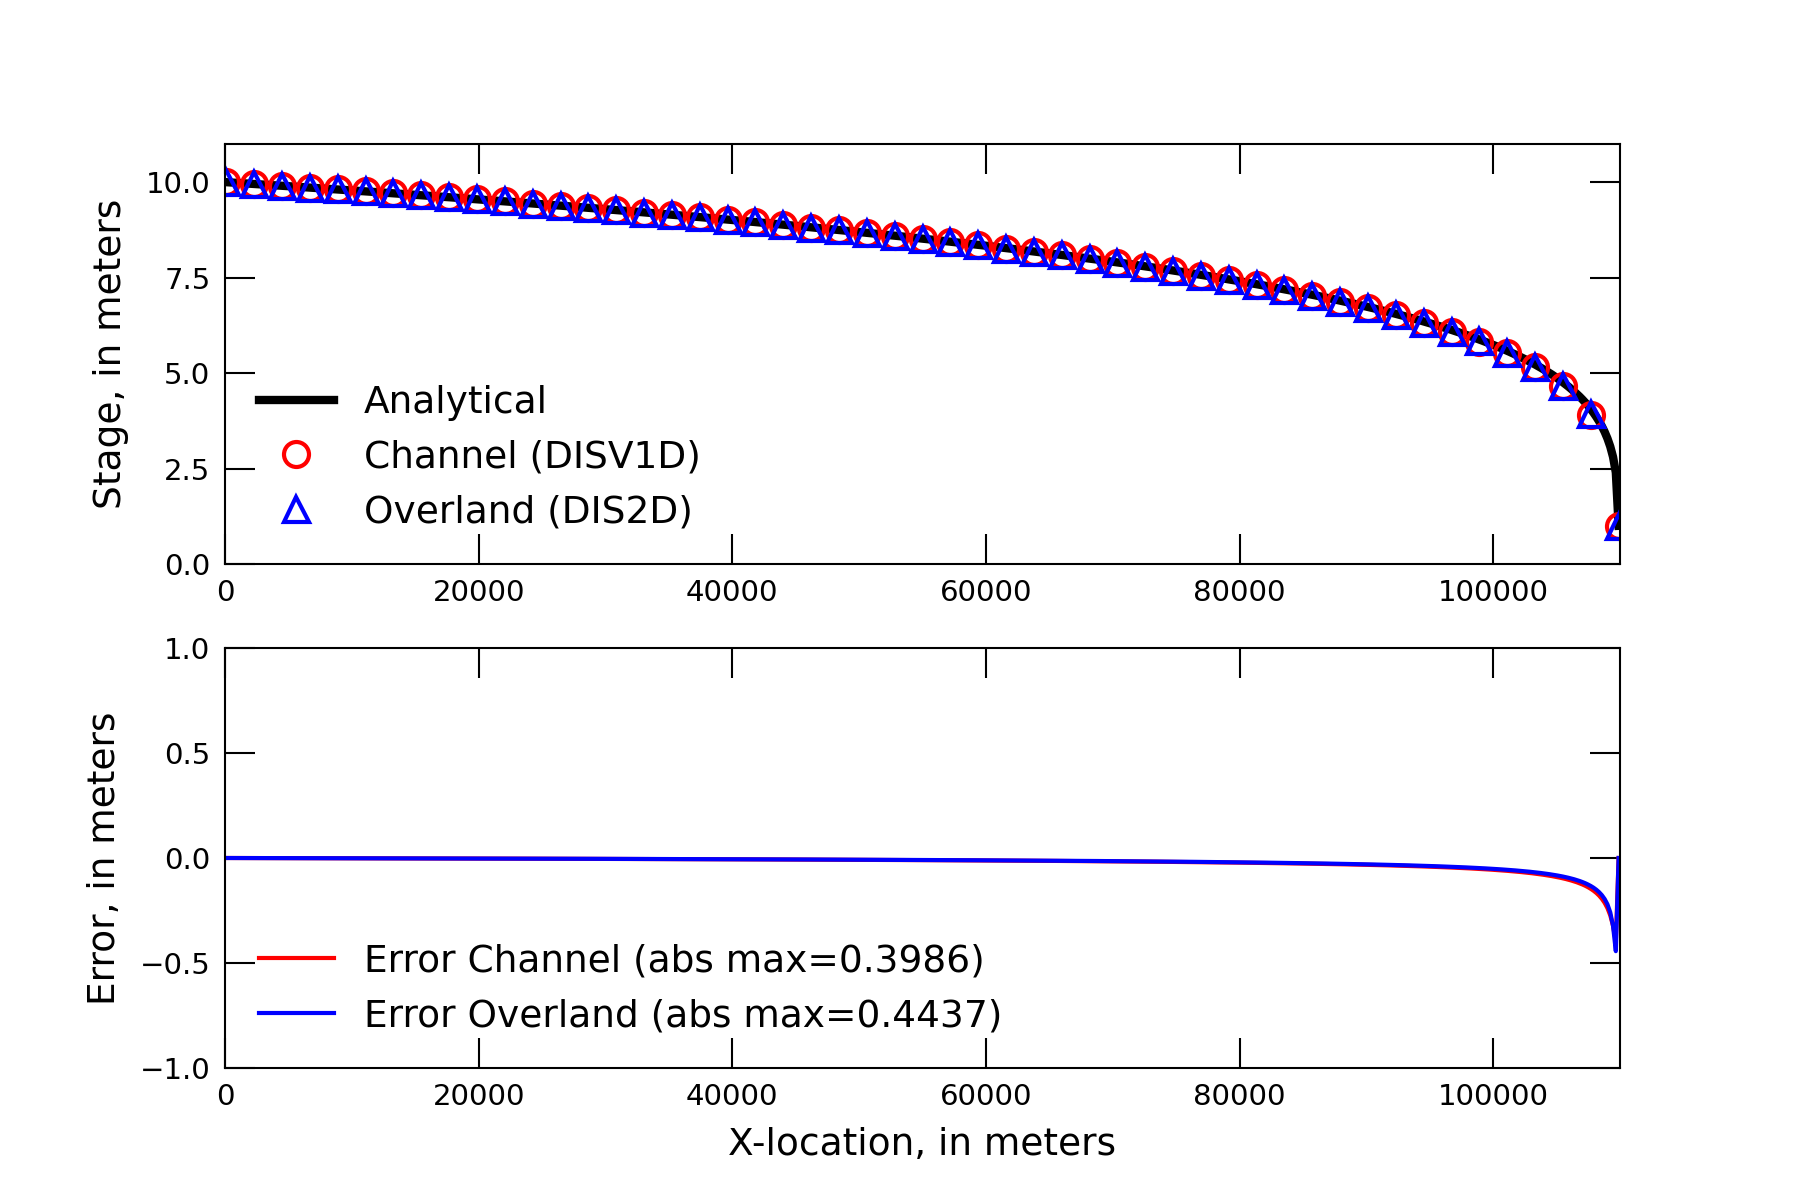
\includegraphics[scale=1.0]{figures/oned.png}
	\caption[Results for one-dimensional flow.]{Results for one-dimensional flow.  Two different Surface Water Flow (SWF) Models are shown.  The channel model represents flow using the one-dimensional DISV1D discretization.  The overland model represents flow using the two-dimensional DIS2D discretization with a single row.}
	\label{fig:oned-results}
\end{figure}

\newpage
\subsection{Steady Radial Flow}

% background
To further demonstrate and test the SWF Model, an analytical solution was also developed for steady one-dimensional radial flow.  Following the previous example, if the bed is level at elevation $z = 0$ and the depth is equal to the stage ($d = h$), then the governing equation for one-dimensional radial surface water flow is

\begin{equation}
  \frac{\partial h}{\partial t} = \frac{1}{r} \frac{\partial}{\partial r} 
  \left (r \frac{h^{5/3}}{n \left | \frac{\partial h}{\partial r} \right |^{1/2}} 
  \frac{\partial h}{\partial r} \right ) = 0 .
\end{equation}

\noindent For flow between two prescribed stage boundaries, with stages of $h_0$ and $h_1$ at radial distances of $r_0$ and $r_1$, respectively, the analytical solution for $h$ as a function of radial distance $r$ is

\begin{equation}
  h = \left [ \left (1 - \rho \right ) h^{\frac{13}{3}}_{0} + \rho h^{\frac{13}{3}}_{1} \right ]^{\frac{3}{13}} ,
  \label{eqn:radial-flow-analytical}
\end{equation}

\noindent where

\begin{equation}
  \rho \equiv \frac{\frac{1}{r_{0}} - \frac{1}{r}}{\frac{1}{r_{0}} - \frac{1}{r_{1}}} .
  \label{eqn:rho_defined}
\end{equation}

% purpose and expectation
In this example, two different model grids are used to simulate steady overland flow and the water surface profile between two prescribed stage boundaries.  Results from the numerical models should be in agreement with the analytical solution.  Some minor differences are expected due to upstream weighting and discretization errors in the numerical model.

%problem description
A structured two-dimensional model grid is represented using the DIS2D discretization package (figure~\ref{fig:oned-structured-grid}).  The DIS2D grid consistes of 151 rows and 151 columns.  Constant heads are assigned to the group of nine model cells in the middle of the domain and around the perimeter of the domain.  The constant head values are calculated using the analytical solution for radial flow (equation \ref{eqn:radial-flow-analytical}).

\begin{figure}[h!tbp]
	\centering
	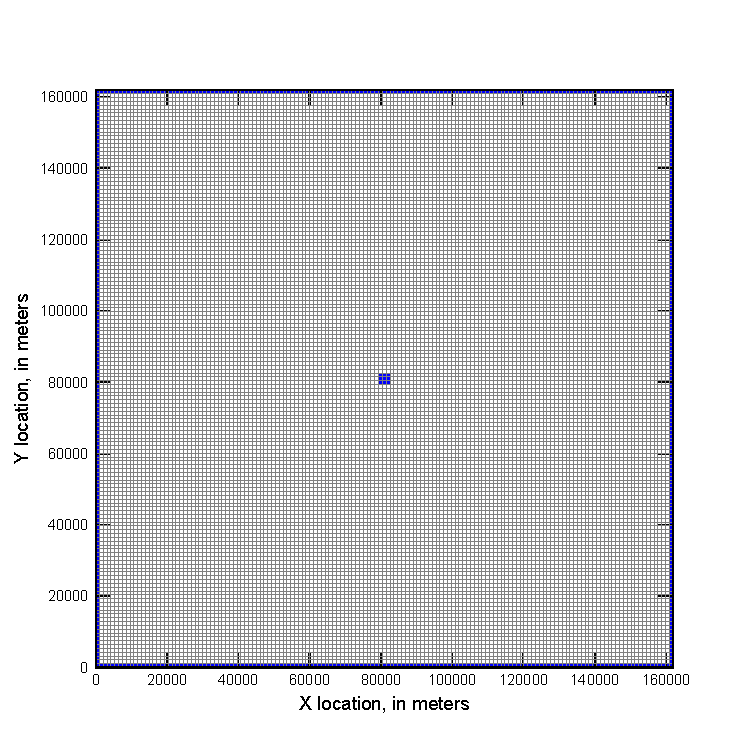
\includegraphics[scale=0.70]{figures/oned-structured-grid.pdf}
	\caption[Structured model grid used to simulate radial flow.]{Structured model grid used to simulate radial flow.  Grid consists of 151 rows and 151 columns.  The model domain spans 162,000 meters in both the x and y directions.  Constant head cells are shown in blue.  Head values for the constant head cells are calculated using the radial flow analytical solution (equation \ref{eqn:radial-flow-analytical}).}
	\label{fig:oned-structured-grid}
\end{figure}

A voronoi model grid, represented using the DISV2D discretization package, is also used to simulate radial overland flow (figure~\ref{fig:oned-voronoi-grid}).  The voronoi model grid was constructed using an inner radius of 5000 m and an outer radius of 80,000 m.  Cells within the gridded domain are no larger than $(5000 m)^2$ in area.  Constant heads are assigned to the ring of innermost cells and outmost cells.  Head values for the constant head cells are calculated using the radial flow analytical solution (equation \ref{eqn:radial-flow-analytical}).

\begin{figure}[h!tbp]
	\centering
	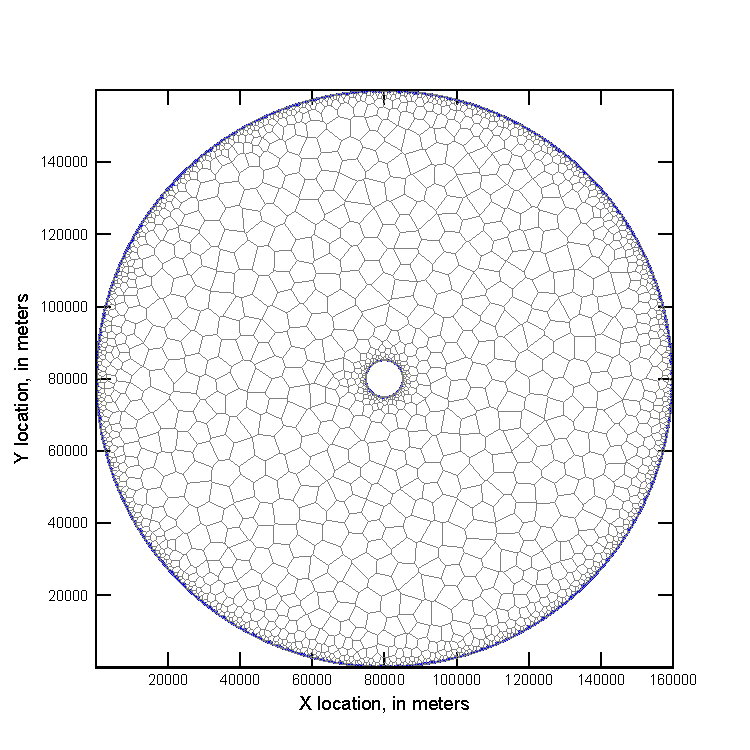
\includegraphics[scale=0.70]{figures/oned-voronoi-grid.pdf}
	\caption[Voronoi unstructured model grid used to simulate radial flow.]{Voronoi unstructured model grid used to simulate radial flow.  Grid consists of 2392 model cells and 6169 vertices.  The radius of the inner circle is 5000 meters, and the radius of the outer circle is 80,000 meters.  Constant head cells, shown in blue, are assigned to the innermost cells and the outermost cells.  Head values for the constant head cells are calculated using the radial flow analytical solution.}
	\label{fig:oned-voronoi-grid}
\end{figure}

%results
The comparison between the analytical solution (equation~\ref{eqn:radial-flow-analytical}) and the simulation with the structured model grid is shown in figure~\ref{fig:oned-structured-results}.  The comparison between the analytical solution (equation~\ref{eqn:radial-flow-analytical}) and the simulation with the voronoi model grid is shown in figure~\ref{fig:oned-voronoi-results}.  In both cases, the simulation results are in good agreement with the analytical solution.

\begin{figure}[h!tbp]
	\centering
	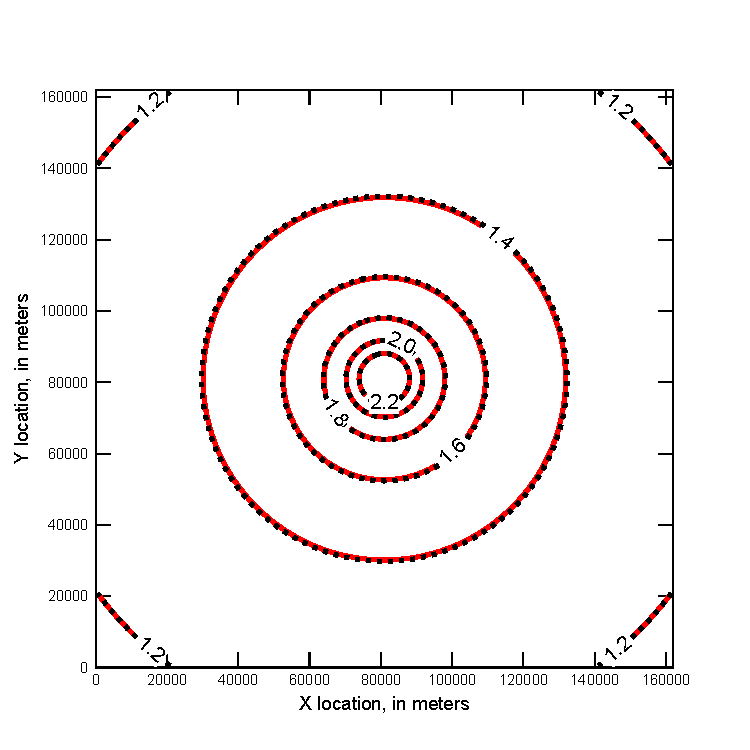
\includegraphics[scale=0.9]{figures/oned-structured-results.pdf}
	\caption[Simulation results from the structured grid model.]{Simulation results from the structured grid model.  Black dotted contours are for the numerical model and the red solid contours are for the analytical solution.  The contour interval is 0.2 meters.}
	\label{fig:oned-structured-results}
\end{figure}

\begin{figure}[h!tbp]
	\centering
	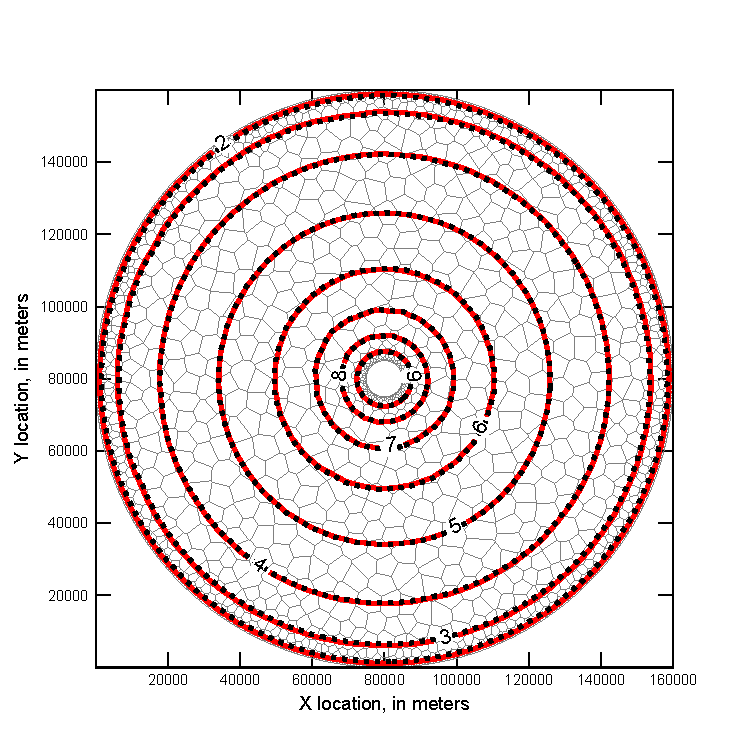
\includegraphics[scale=0.9]{figures/oned-voronoi-results.pdf}
	\caption[Simulation results from the voronoi grid model.]{Simulation results from the voronoi grid model.  Black dotted contours are for the numerical model and the red solid contours are for the analytical solution.  The contour interval is 1.0 meters.}
	\label{fig:oned-voronoi-results}
\end{figure}

\newpage
\subsection{Axisymmetric Overland Flow}

The axisymmetric flopy problem developed by~\cite{lal2001}, and used by~\cite{hughes2015} to test the SWR Process for MODFLOW-2005, is used to test the SWF Model for MODFLOW 6.  The problem is based on the transient decay of a circular mound of surface water.

\begin{figure}[h!tbp]
	\centering
	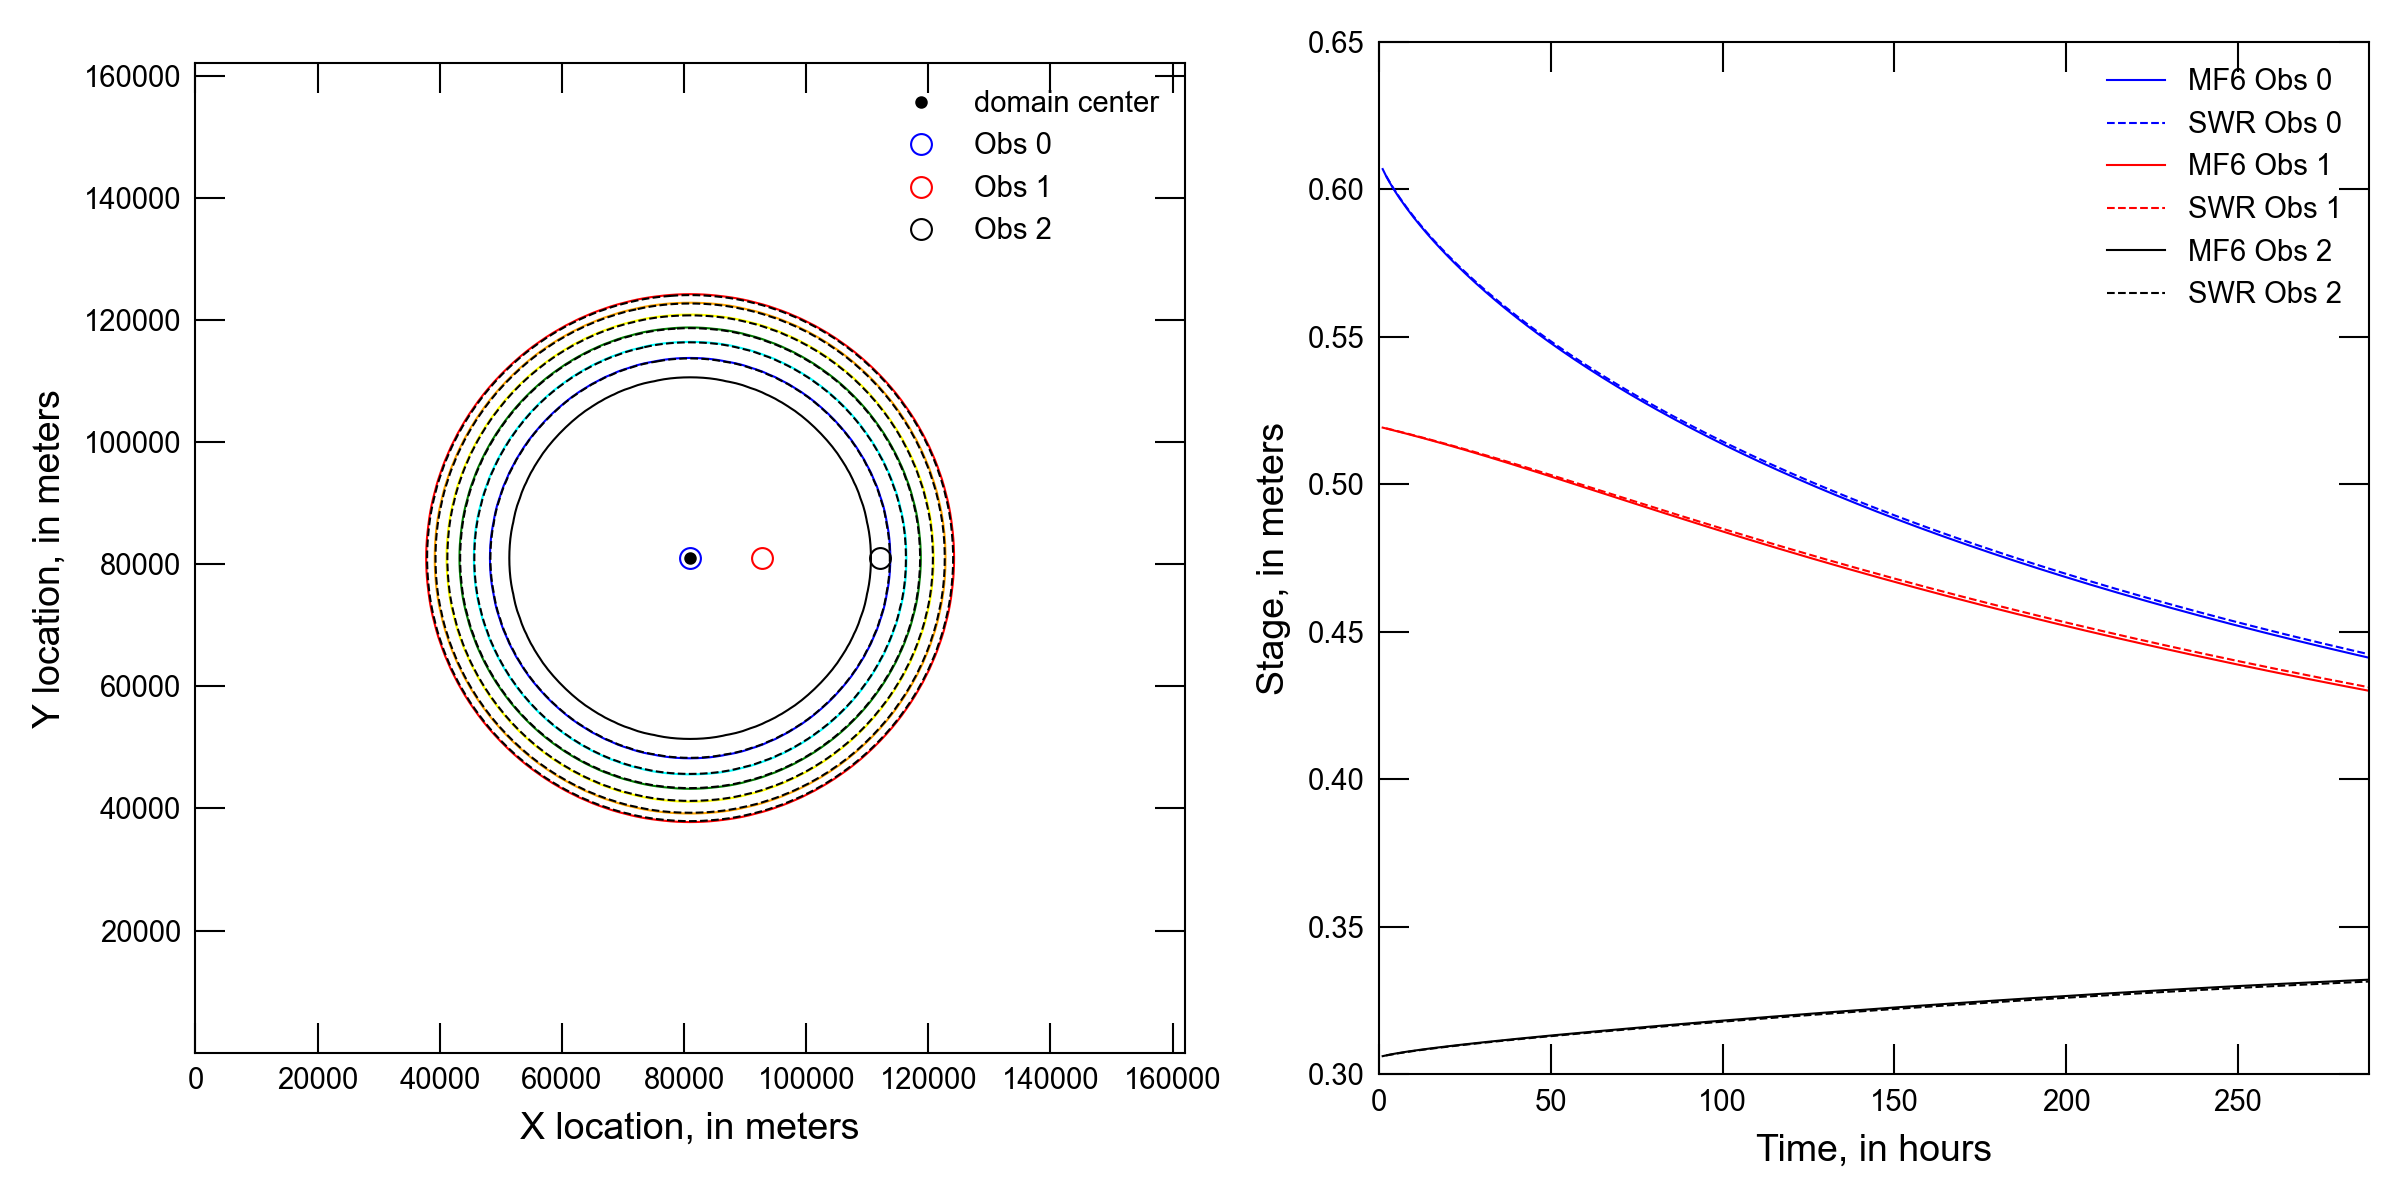
\includegraphics[scale=0.70]{figures/axi-results.png}
	\caption[Simulation results for the axisymmetric overland flow problem.]{Simulation results for the axisymmetric overland flow problem.}
	\label{fig:axi-results}
\end{figure}

\newpage
\subsection{Tilted V-Catchment}

The MODFLOW 6 SWF Model was used to simulate the tilted V-catchment problem described by \cite{digiammarco1996}.  This tilted V-catchment problem has been used by~\cite{VanderKwaak1999},~\cite{panday2004} and by~\cite{hughes2015}, for example, to test numerical models of two-dimensional overland in response to a rainfall event.

The configuration of the tilted V-catchment is shown in Figure~\ref{fig:vcatch-surface}.  The left and right sides of the domain consist of sloping flat planes.  The flat planes are tilted to the south and toward the middle of the domain, forming a V-shaped catchment.  A slope of 0.05 is used for the x direction, and a slope of 0.02 is used for the y direction.  Located between the two sloping planes is a 20-m wide stream channel that slopes from north to south.  Two different Mannings roughness coefficients are used.  A value of 0.015 is assigned to the sloping planes and a value of 0.15 is assigned to the stream channel.  These values are not realistic, in that roughness coefficients are generally lower within a stream channel compared to sloping surfaces, but they were selected as a difficult test for simulating overland flow.  A zero-depth gradient boundary condition assigned as the southernmost part of the stream provides the sole outlet for the domain.

\begin{figure}[h!tbp]
	\centering
	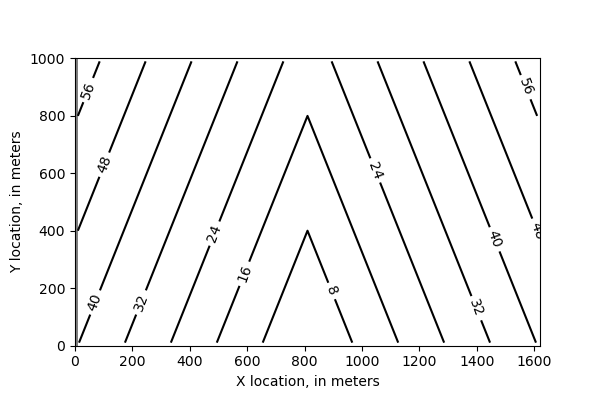
\includegraphics[scale=0.75]{figures/vcatch-surface.png}
	\caption[Configuration of the tilted v-catchment example.]{Configuration of the tilted v-catchment example.  Contours represent land surface.  A slope of 0.05 is used for the x direction, and a slope of 0.02 is used for the y direction.  A 20-m wide stream channel, shown in gray, slopes from north to south.}
	\label{fig:vcatch-surface}
\end{figure}

The domain is discretized into a regular model grid consisting of 50 rows and 81 columns.  Each cell is square with a dimension of 20 m.  Rainfall is uniformly applied to the domain at a rate of $3 \times 10^{-6}$ for a period of 90 minutes.  A second 90-minute period with no rainfall is also represented to simulate drainage of the domain in response to the rainfall event.  Following the settings used by~\cite{panday2004} adaptive time stepping is used with an inital time step of 5 s and a maximum time step of 100 s.  Time steps increase or decrease by a factor of two in response to solver behavior.

Results from the MODFLOW 6 SWF Model simulation are compared in Figure~\ref{fig:vcatch} with the simulations results of~\cite{digiammarco1996},~\cite{VanderKwaak1999},~\cite{panday2004} and~\cite{hughes2015}.  In general, the model results from MODFLOW 6 compare favorably with the results from these other models; however, rates of simulated outflow from the MODFLOW 6 simulation rise and fall more quickly than for the other models.

\begin{figure}
	\centering
	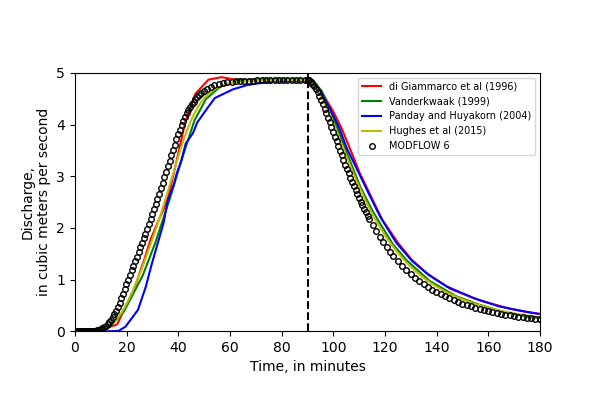
\includegraphics[scale=0.75]{figures/vcatch-results.png}
	\caption[Simulated discharge for the tilted v-catchment example.]{Simulated discharge for the tilted v-catchment example.  Dashed blue line separates the first 90-minute period with rainfall from the second 90-minute period with no rainfall.}
	\label{fig:vcatch}
\end{figure}

% \subsection{Tilted V-Catchment with Aquifer Exchange}
% \cite{panday2004} modified the tilted v-catchment problem to include an underlying aquifer.  Flow in their underlying aquifer was represented using Richards equation in order to represent unsaturated flow.  Given that MODFLOW 6 does not have a Richards formulation, this problem was represented using a single aquifer layer with the unconfined flow equation.

\subsection{Modified Pinder-Sauer}
\cite{pindersauer1971} evaluated the effect of bank storage on flood wave propagation.  As part of their analysis, they developed a numerical model of coupled surface and groundwater flow.  \cite{swainwexler1996} used the test problem reported by \cite{pindersauer1971} to verify that the MODBRANCH program was working properly.  The \cite{pindersauer1971} problem was modified by \cite{lal2001} so that an analytical solution could be derived to represent the surface and groundwater exchange.  The modified Pinder-Sauer problem has been used by \cite{lal2001} and by \cite{hughes2015} to test the accuracy of numerical codes for representing surface and groundwater exchange.  

The modifed Pinder-Sauer problem is used here to test the coupling of the SWF and GWF numerical models.  Results from the integrated simulation are compared with the analytical solution of \cite{lal2001}.  A regular structured grid is used for the SWF and GWF models.  The model dimensions in the x and y directions are 427 m and 39624 m, respectively.  There are 65 rows and 15 columns.  A spacing of 28.3 m is used for all columns, except column 8, which is assigned a spacing of 30.48 m.  A spacing of 609.61 m is used for all rows.  The land surface slopes downward from a value of 67.05 m at the top end to an elevation of 27.43 at the bottom end.  This slope corresponds to 0.001.  The GWF model consists of one layer.  The top of the GWF model corresponds to land surface and the bottom of the GWF model has a constant elevation of 0 m.

For the SWF model, only column 8 is active.  All of the SWF cells in columns one through 7 and 9 through 15 are assigned an IDOMAIN value of 0.  Inflow to the SWF model in row 1 and column 7 is assigned ased on the following equation

\begin{equation}
  Q_{in} = 509.70 + 141.58 sin \left ( \frac{2 \pi t}{T_p} \right )
\end{equation}

\noindent where $Q_{in}$ is the inflow to the SWF Model in $m^3/s$, $t$ is time in seconds, and $T_p$ is the wave period, specified to be 18,000 seconds (5 hours).  A zero-depth gradient boundary was assigned to the last row in column 8 to allow surface water to flow out freely.  Thus, surface water flows from the top end of the model to the bottom end in column 7 and exchanges with the underlying aquifer along the way.  No-flow conditions are prescribed around the entire perimeter of the GWF Model.

The Mannings roughness coefficient was assigned a value of 0.03858 $s/m^{1/3}$.  For the GWF Model a value of $3.048 \times 10^{-3}$ $m/s$ was assigned for hydraulic conductivity. The GWF Model is treated as confined with a specific storage value of 0.25 $1/m$.  The leakage coefficient representing the exchange property between the SWF and GWF Models was set to $1.402 \times 10^{-4}$ $1/s$.

The initial depth of water in column 8 of the SWF Model was set to 6.09 m, thus giving a sloping water surface that decreases from top to bottom.  This sloping water surface elevation was also used as the starting head for the GWF Model.  The simulation period of 24 hours was evenly divided into 288 equally sized 5 minute time steps.  

The analytical solution for this problem, as given by \cite{lal2001}, is

\begin{equation}
  Q_{in} = 509.70 + 141.58 
  exp \left ( \frac{\lambda_1 x}{\Lambda} \right ) 
  sin \left ( f_r t + \frac{\lambda_2 x}{\Lambda}\right ),
\end{equation}

\noindent where for the case with leakage, $\lambda_1$ is -0.1785, $\Lambda$ is 4894.3 m, $f_r$ is $3.49 \times 10^{-4}$, and $\lambda_2$ is -0.3409.  For the case without leakage, $\lambda_1$ is -0.04799 and $\lambda_2$ is -0.3608.

The simulation was run with and without leakage.  Results from the SWF Model for flow between row 25 and row 26 in column 8 are compared with the analytical solution (Figure \ref{fig:pinder-sauer}). After a brief spin-up period, the results from MODFLOW are in good agreement with the results from the analytical solution.

\begin{figure}
	\centering
	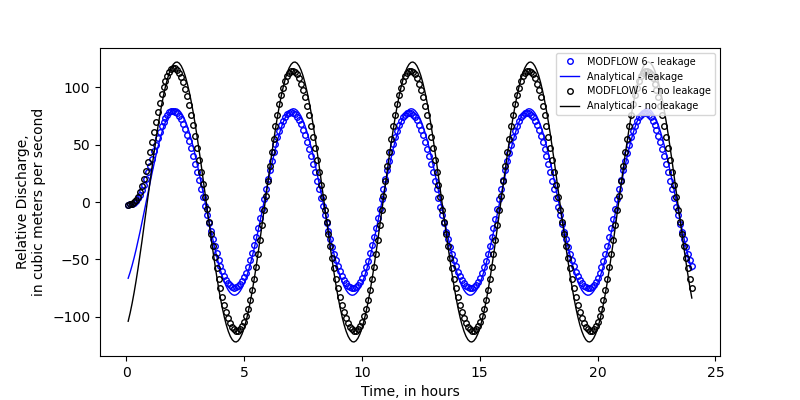
\includegraphics[scale=0.50]{figures/pinder-sauer-results.png}
	\caption[Simulated discharge between row 25 and row 26 in column 8 for the modified Pinder-Sauer problem.]{Simulated discharge between row 25 and row 26 in column 8 for the modified Pinder-Sauer problem.}
	\label{fig:pinder-sauer}
\end{figure}


% \bibliographystyle{plain}
\bibliographystyle{apalike}
\bibliography{swfref} 

\end{document}